%% ------------------------------------------------------------------------- %%
\chapter{Tecnologias}
\label{cap:tecnologias}
\section{Ruby on Rails}
\subsection{Ruby}
    \par A criação da linguagem Ruby data de 1995 no Japão por Yukihiro "Matz" Matsumoto sob forte influência de outras linguagens como Perl, SmallTalk, Eiffel, Ada e Lisp.
    \par Inicialmente o objetivo era equilibrar programação funcional, imperativa e orientação a objetos. Segundo o próprio Matz: "Eu queria uma linguagem interpretada que fosse mais poderosa do que Perl e mais orientada à objetos do que Python2." (\cite{rubydocs}).
\begin{itemize}
\item{Flexibilidade:}
    \par A Linguagem Ruby cresceu devido a sua grande flexibilidade. Sendo possível alterar, remover ou acrescentar partes da linguagem à vontade.
    \par Imagine o seguinte exemplo: um usuário prefere utilizar a palavra \par{plus} ao invés do operador matemático(  +  ), ele poderia então adicionar esse método à classe nativa do Ruby Numeric pois em ruby os operadores matemáticos são considerados açúcares sintáticos.
\\Exemplo:
\begin{lstlisting}[frame=single]
class Numeric
          def plus(x)
                self.+(x)
          end
    end

    y = 5.plus 6
    # y agora eh igual a 11
\end{lstlisting}
\item{Closures:}
    \par Nesta linguagem, \emph{closures} são chamadas de blocos e são funções que podem ser tratadas como uma variável.
    \par Isso quer dizer que podem ser passadas como argumentos de métodos, serem atribuídas a outras variáveis, etc.
    \par As \emph{closures} armazenam os valores das variáveis que estavam no escopo quando a função foi definida e são capazes de acessar tais variáveis mesmo que sejam executadas em um escopo diferente. \footnote{Fonte: Site Point \url{https://www.sitepoint.com/closures-ruby/}}
\\
Exemplo:
\begin{lstlisting}[frame=single]
search_engines =
  %w[Google Yahoo MSN].map do |engine|
    "http://www." + engine.downcase + ".com"
  end
\end{lstlisting}
\item{Módulos:}
    \par Diferente de outras linguagens orientadas a objetos o Ruby suporta apenas herança simples porém de forma proposital.
    \par O conceito de módulos que são coleções de métodos que podem ser adicionadas à uma classe por meio de um \emph{mixin}.
    \par As classes podem fazer o mixin de um método e receber todos os métodos dele diretamente.
Exemplo:
\begin{lstlisting}[frame=single]
class MyArray
          include Enumerable
    end
\end{lstlisting}

\end{itemize}
\subsection{Rails}

\par Ruby on Rails é um arcabouço escrito em linguagem Ruby, implementado seguindo o padrão MVC\footnote{Modelo-Visão-Controlador: Na qual o Modelo é a camada contém os dados e lógica da aplicação, a Visão é camada de entrada e saída de dados e o Controlador faz a conexão entre ambas camadas, fonte: \url{https://pt.wikipedia.org/wiki/MVC} } totalmente \emph{server-side}, sendo considerado portanto um arcabouço \emph{ back-end}.
\par David Heinemeier Hansson, criador da tecnologia, extraiu o Ruby on Rails do seu próprio trabalho realizado na empresa Basecamp e foi lançado como código-aberto pela primeira vez em 2004.
\par Este \emph{framework} oferece também uma estrutura para banco de dados \emph{web service} e \emph{web pages}, além de encorajar padrões de engenharia de software já consagrados tais como:(\cite{railswiki})
\begin{itemize}
\item {\emph{Convention over Configuration} (CoC):}
    \par Convenções de configuração visando padronizar o código. Ao adicionar convenções é retirada do desenvolvedor a decisão de como usar o arcabouço porém isso não diminui sua flexibilidade. Por exemplo se existir um objeto chamado "User" então sua tabela por convenção se chamará "users" e correspondente \emph{controller} será UsersController ( no plural) pois esse é padrão definido pelo arcabouço mas é possível alterar essas convenções para adaptar-se às necessidades do desenvolvedor.

\item {\emph{Don't Repeat yourself} (DRY):}
    \par É definido como "Todo pedaço de informação deve ter uma única, não ambígua, representação autorizada com o Sistema" \footnote{Fonte: Wikipedia \url{https://en.wikipedia.org/wiki/Don\%27t_repeat_yourself}}.
    \par Isso significa que uma modificação em uma parte do sistema não deve modificar outra parte não relacionada assim como elementos que são logicamente relacionados quando modificados ocorrem de forma previsível e uniforme.

\item { \emph{Active Record Pattern}:}
    \par O padrão Active Record sugere uma interface específica para acessar objetos em um banco de dados relacional contendo funções tais como INSERT, UPDATE, DELETE, etc.
    \par Uma tabela ou \emph{view} será associada a uma classe e então uma instância de objeto estará associada a uma única entrada na respectiva tabela.
    \par Em Ruby on Rails a biblioteca ActiveRecord implementa o padrão ORM e além disso acrescenta herança e associações, resolvendo dois problemas substanciais do padrão.
    \par ActiveRecord é o "model" padrão do componente MVC porém é possível trocá-lo por outra implementação do arcabouço Rails caso o desenvolvedor prefira.
\end{itemize}
    \par Em um sentido mais amplo Rails é mais que uma biblioteca de software ou API: é um projeto central de uma vasta comunidade que produz \emph{plugins} para facilitar e construir projetos complexos de web site.
    \par Foi graças a essa comunidade que compartilham ferramentas e contribuem para o projeto Rails criando bibliotecas em código aberto ( chamadas de Ruby Gems ou apenas Gems \footnote{Fonte: Wikipedia \url{https://en.wikipedia.org/wiki/RubyGems}}) que o o uso de rails tem crescido de forma significante nos últimos anos ganhando fama entre startups devido a sua  facilidade e desevolvimento que permite criar sistemas complexos e testar idéias rapidamente.

\section{Heroku}
\par Heroku é uma Paas implementada utilizando \emph{cloud computing} criada em 2007 utilizada como um modelo de \emph{Deployment} para Aplicações Web. ( \cite{herokuwiki})
\par A rede do Heroku roda os aplicativos em containers virtuais. Esses containers são chamados de Dynos e podem rodar códigos escritos em Nodejs, Ruby, PHP, Go, Scala, Python, Java, Clojure.
\par A aplicação é enviada para o Heroku por meio de uma conexão direta via GitHub, Dropbox ou alguma API.
\par Enviado o código-fonte ele então é convertido em uma aplicação interpretando as dependências de outras bibliotecas seguindo o padrão de cada linguagem. No caso do USP Eventos que foi feito utilizando Ruby as dependências ficam armazenadas no próprio Gemfile da aplicação.
\par Feito o \emph{upload} da aplicação um container com uma virtualização de Unix é disponibilizado, o Dyno da aplicação. Tal container é pré-carregado com algumas configurações prévias da aplicação: um nome gerado automaticamente, variáveis de ambiente e \emph{add-ons} se existirem.
\par O Heroku então inicializa o Dyno com a aplicação, carrega-a e então realiza o \emph{deploy} da mesma.
\par Através do DNS Server oferecido pelo próprio Heroku a aplicação fica acessível por meio de um domínio na forma <nome da aplicação>.herokuapp.com sendo possível redirecionar seu domínio particular para refletir o DNS disponibilizado.
\section{Travis CI}
\par Travis CI é um serviço de integração contínua usado para testar projetos hospedados no Github.
\par Toda vez que um commit para o repositório selecionado no Gitbhub o Travis irá executar as diretrizes especificadas no arquivo travis.yml que contém os comandos necessários para rodar os testes automatizados da aplicação, como é o caso do USP Eventos (figura \ref{fig:travis}).
\begin{figure}[htb]
\centering
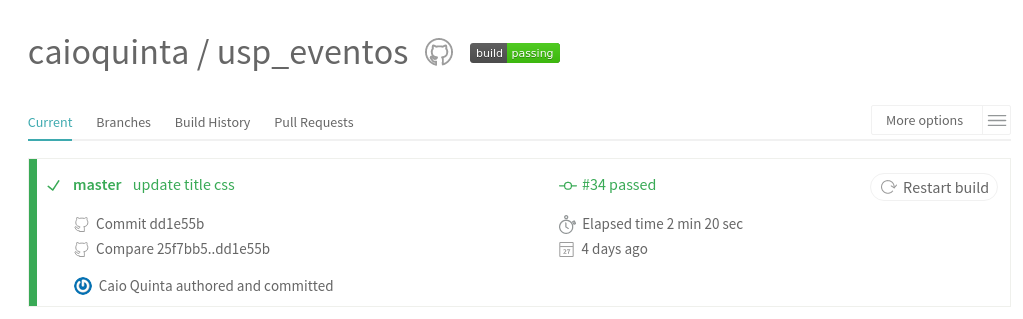
\includegraphics[width=15cm]{figuras/travis}
\caption{\label{fig:travis} O repositório USP Eventos no Travis CI.}
\end{figure}

\section{Trello}
\par Trello é um gerenciador de projetos online desenvolvido pela Fog Creek Software lançado em 2011.
\par Possui uma interface amigável na qual é possível criar tarefas e colunas conforme as preferências do usuário sendo bastante utilizado em conjunto com uma abordagem \emph{kanbam} para gerenciamento.

\section{Github}
\par Github é um repositório git baseado na web lançado em 2008.
\par Ele oferece um serviço de controle de versão que provê todas as funcionalidades do Git assim como outras funcionalidades próprias como gerenciamento de tarefas, wikis próprias e \emph{bug tracking}.
\par Atualmente diversos outros serviços oferecem a opção de integração com o Github por meio de uma API.
\par No caso do USP Eventos a integração com o Github foi feita dentro do Travis CI para efetuar o processo de integração contínua.
\par Além disso o Heroku também era integrado com o Github sendo que quando um \emph{commit} era feito para o repositório com o nome de "Produção" e o mesmo fosse aprovado em todos os testes pelo Travis CI o deploy da aplicação era realizado automaticamente.
\par Tal integração entre o Heroku (figura \ref{fig:heroku_automatic_deploy}) e o Travis CI só foi possível graças a utilização do Github.
\begin{figure}[htb]
\centering
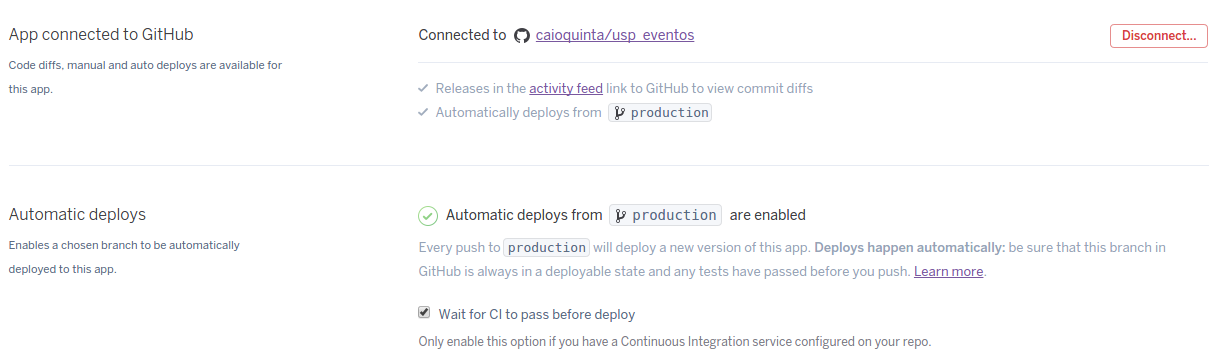
\includegraphics[width=15cm]{figuras/heroku_automatic_deploy}
\caption{\label{fig:heroku_automatic_deploy} Tela de Administração do Heroku para integração com o Github e Deploy automático.}
\end{figure}
\section{Google Analytics e Google Tag Manager}
\par O google Analytics é uma plataforma de análise de dados oferecida pelo Google.
\par Por meio dos relatórios gerados pela plataforma é possível obter uma série de informações quanto ao tipo de usuário que visualiza a página, o fluxo do site e a origem do acesso.
\par Através de \emph{tags} configuráveis é possível criar eventos que são personalizados e disparados de acordo com a navegação do usuário dentro do site.
\par Tais \emph{tags} podem ser implementadas diretamente através de um pequeno código em javascript para integração com o Google Analytics ou utilizando o Google Tag Manager.
\par O Google Tag Manager é uma plataforma intermediária que provê acesso e configuração de tags personalizadas para obtenção de dados pelo Google Analytics sem que seja necessário modificar diretamente o código-fonte do sistema.
\par A opção de utilizar o Google Tag Manager no projeto deu-se principalmente pela facilidade de criar-se novas tags e alterações além de garantir uma maior organização das informações.
\par Dentro do projeto utilizamos as informações obtidas através do Google Analytics para validação de aprendizado entre as interações.

\section{Painel de opiniões Populares - POP}
\par Com o intuito de definir o interesse do público alvo por meio de uma enquete colaborativa utilizamos o POP como sistema de votação devido a possibilidade dos usuários poderem adicionar adicionar itens à enquete principal.
\par Desenvolvido por estudantes do próprio IME dentro da disciplina de Laboratório de Programação Extrema à pedido da INDX o POP é uma plataforma de pesquisa de opinião pública que possui o objetivo realizar enquetes junto à comunidades para auxiliar na tomada de decisões e encaminhamento de opiniões para as autoridades responsáveis.
\par Foi permitida a utilização da plataforma implementada em uma instância separada com o nome de POP-TCC. para realização da enquete junto à comunidade USP para definir qual seria o tema do projeto.
\par Uma pequena modificação no sistema POP original foi feita para o POP-TCC.
\par No POP-TCC os usuários só poderiam votar de maneira positiva nas opções ao contrário do sistema original que permitia votos negativos e até ocultamento dos itens que fossem muito negativados pelos usuários.

\section{HeatMap}
\par O serviço fornecido pela plataforma Heatmap.me consiste em prover uma API que é capaz de capturar os cliques em uma determinada página e mostrá-los na forma de uma mapa de calor.
\par Um mapa de calor é uma representação gráfica dos cliques em uma página na qual conforme uma determinada região for recebendo mais cliques sua cor é alterada proporcionalmente(figura \ref{fig:heatmap_explanation}).
\begin{figure}[htb]
\centering
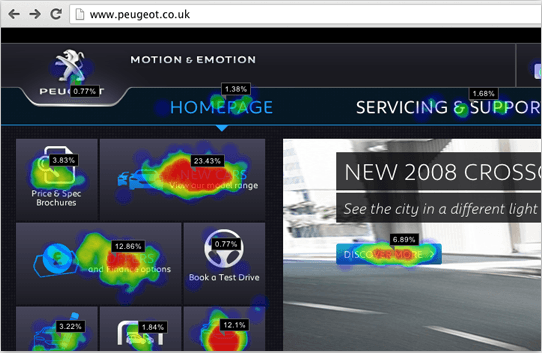
\includegraphics[width=15cm]{figuras/heatmap_explanation}
\caption{\label{fig:heatmap_explanation} Um exemplo de uma página utilizando o HeatMap.}
\end{figure}
\par As cores inicialmente começam em um tom verde quando clicadas poucas vezes sendo gradativamente alteradas para cores mais "quentes" tais como laranja ou vermelho conforme cliques na mesma região são feitos.

\section{Typeform}
\par A empresa Typeform oferece um serviço de formulários online para execução de pesquisas, simples ou complexas.
\par A ferramenta é ótima para entrevistas de satisfação e opinião do cliente, oferecendo uma interface gráfica bastante amigável além de templates configuráveis para o tipo de pesquisa que o usuário deseja realizar.
\par Após a execução da pesquisa é possível exportar os resultados em planilhas ou integrar com o seu banco de dados caso desejar.
